\chapter{Protótipo}

A prototipação é uma etapa de suma importância no desenvolvimento de projeto de software. Além de melhorar a produtividade da equipe, ela facilita o entendimento dos requisitos do sistema e permite a apresentação de de conceitos e funcionalidades da aplicação de modo simplificado.
Nesse trabalho foi utilizado a prototipação visual cujo ênfase se aplica a estética e usabilidade. Nesse tipo de protótipo é possível identificar o layout e a identidade visual da aplicação. \cite{dextra2013prototipacao}

{Protótipos podem ser gerados de acordo com as seguintes categorias \cite{coyette2004sketchixml}: protótipos em baixa fidelidade que focam na interação, em componentes de interface e na estrutura geral do sistema; protótipos em alta fidelidade que produzem uma imagem real do sistema; protótipos executáveis que produzem o código em uma linguagem de programação, focando em navegação, mas sem ainda levar em consideração as regras de negócio. Cada categoria serve para um propósito específico: protótipos em baixa fidelidade são úteis para demonstrar aos usuários quais atividades o sistema atende e as possibilidades de navegação no sistema, assim como para proporcionar uma visão geral do sistema. Protótipos em alta fidelidade são úteis para demonstrar padrões e guias de estilo. Protótipos executáveis são úteis para demonstrar navegação e testar o uso da interface \cite{rosemberg2008prototipaccao}.Seguindo as definições, o projeto desenvolvido utiliza os protótipos de baixa fidelidade}

\section{Aplicação WEB}
A aplicação web tem como foco o gerenciamento de toda a aplicação envolvendo consultas e cadastros gerais do sistema.
Apesar desse foco acentuado à gestão, é possível desempenhar todos os papeis dentro da aplicação web.

\newpage
\subsection{Login}

\begin{figure}[htb]
	\caption{\label{web_login}Tela de Login do Agil.It}
	\begin{center}
		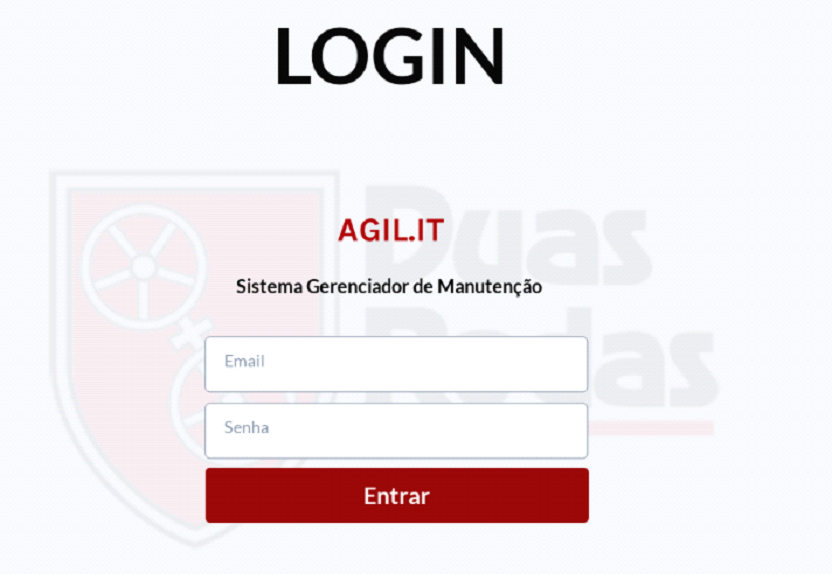
\includegraphics[scale=0.70]{./Figuras/web/login.png}
	\end{center}
	\legend{Fonte: Próprio Autor, 2019}
\end{figure}

A tela \ref{web_login} será a página responsável por autenticar os usuários e garantir a segurança do sistema.

\newpage
\subsection{Cadastro de Ordem de Manutenção}

\begin{figure}[htb]
	\caption{\label{web_cad-om}Cadastro de Ordem de Manutenção}
	\begin{center}
		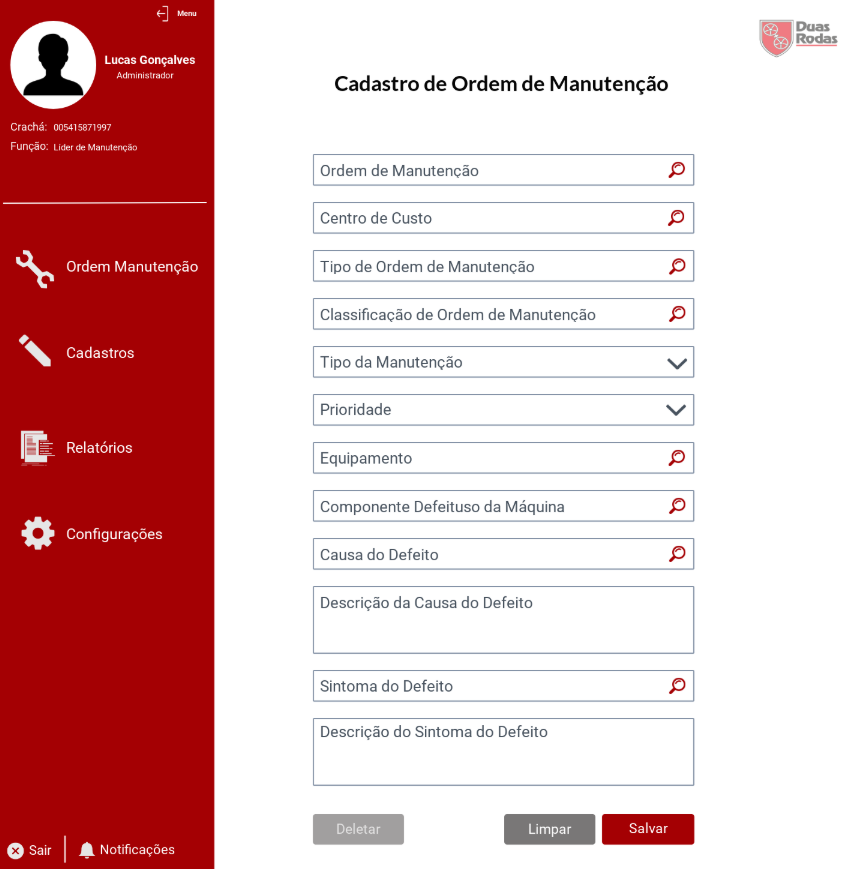
\includegraphics[scale=0.65]{./Figuras/web/cad-om.png}
	\end{center}
	\legend{Fonte: Próprio Autor, 2019}
\end{figure}

Na tela \ref{web_cad-om} é cadastrada e atualizada ordens de manutenção. Ela terá acesso às operações, componentes e assinaturas.

\newpage
\subsection{Monitor de Ordem de Manutenção: Cards}

\begin{figure}[htb]
	\caption{\label{web_monitor-om-card}Monitor de Ordem de Manutenção: Cards}
	\begin{center}
		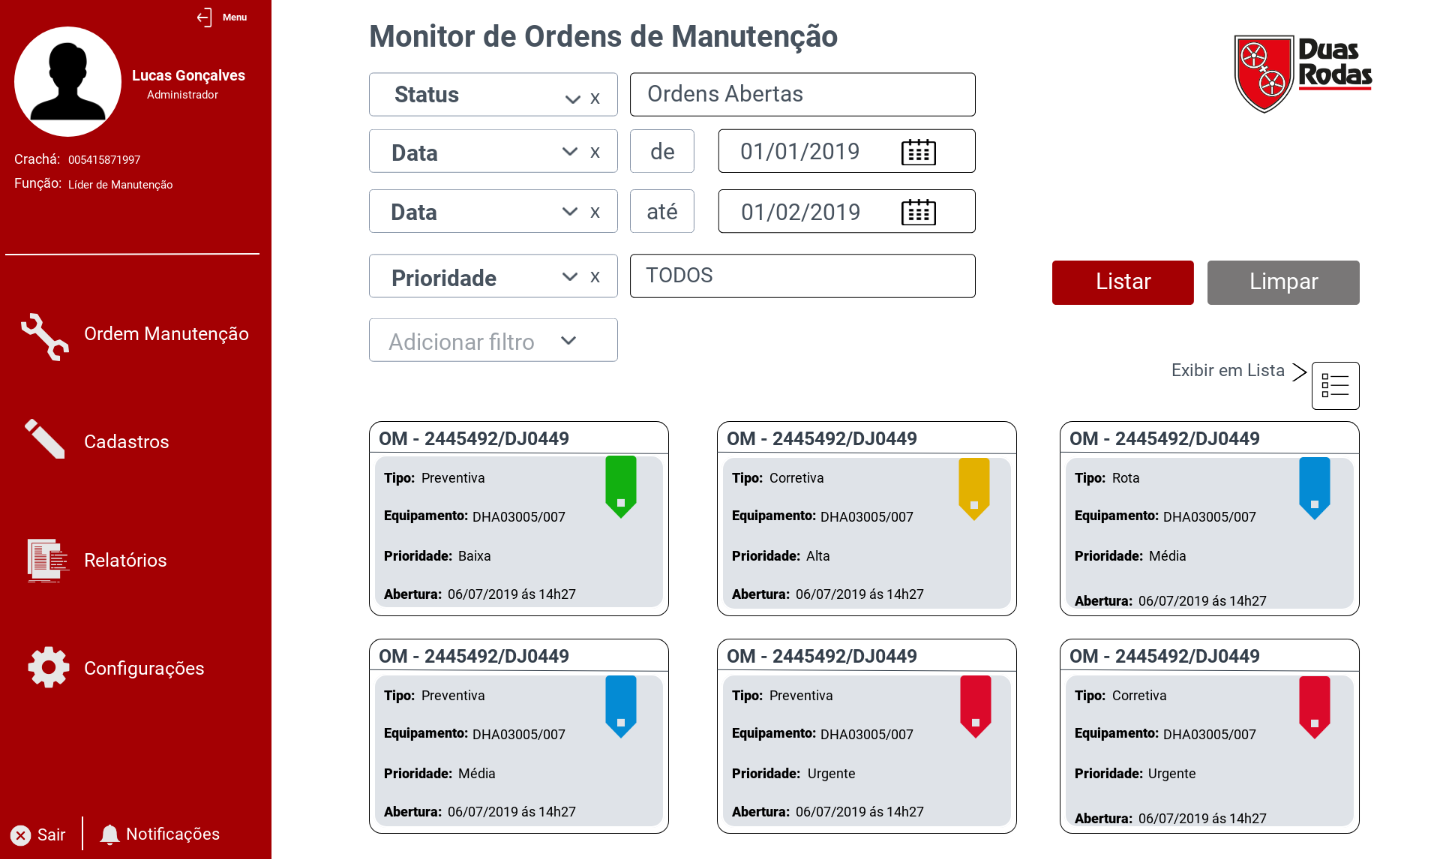
\includegraphics[scale=0.45]{./Figuras/web/monitor-om-card.png}
	\end{center}
	\legend{Fonte: Próprio Autor, 2019}
\end{figure}

A tela \ref{web_monitor-om-card} permite a consulta rápida e dinâmica das ordens de manutenção. Nela você pode aplicar os filtros de acordo com as \newline necessidades e será listada em forma de cartões, eles darão acesso à uma tela de detalhamento de ordem de manutenção.

\newpage
\subsection{Monitor de Ordem de Manutenção: Listas}

\begin{figure}[htb]
	\caption{\label{web_monitor-om-lista}Monitor de Ordem de Manutenção: Listas}
	\begin{center}
		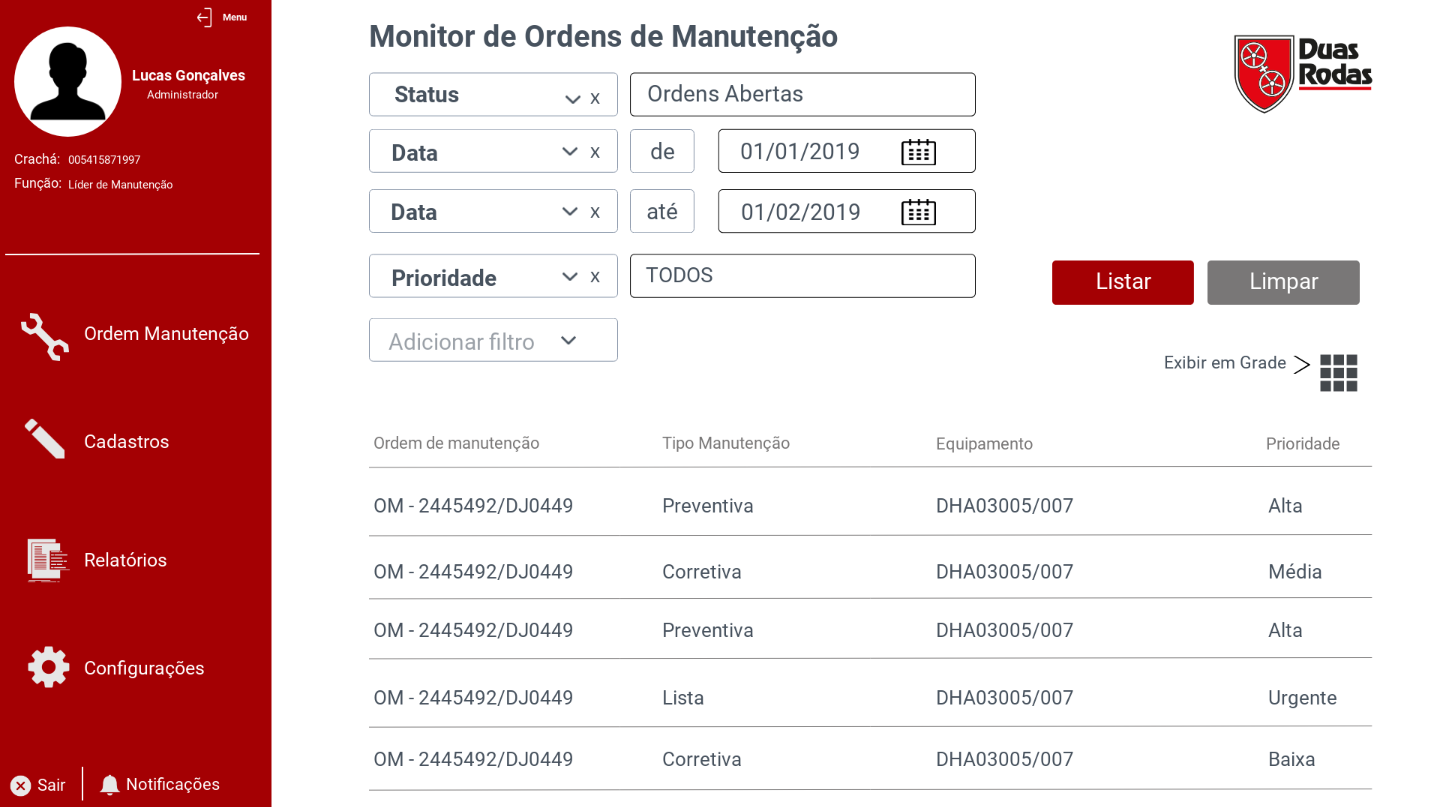
\includegraphics[scale=0.45]{./Figuras/web/monitor-om-lista.png}
	\end{center}
	\legend{Fonte: Próprio Autor, 2019}
\end{figure}

A tela \ref{web_monitor-om-lista} permite a consulta rápida e dinâmica das ordens de manutenção. Nela você pode aplicar os filtros de acordo com as \newline necessidades e será listada em forma de listas, eles darão acesso à uma tela de detalhamento de ordem de manutenção.

\newpage
\subsection{Ordem de Manutenção}

\begin{figure}[htb]
	\caption{\label{web_om-capa}Ordem de Manutenção}
	\begin{center}
		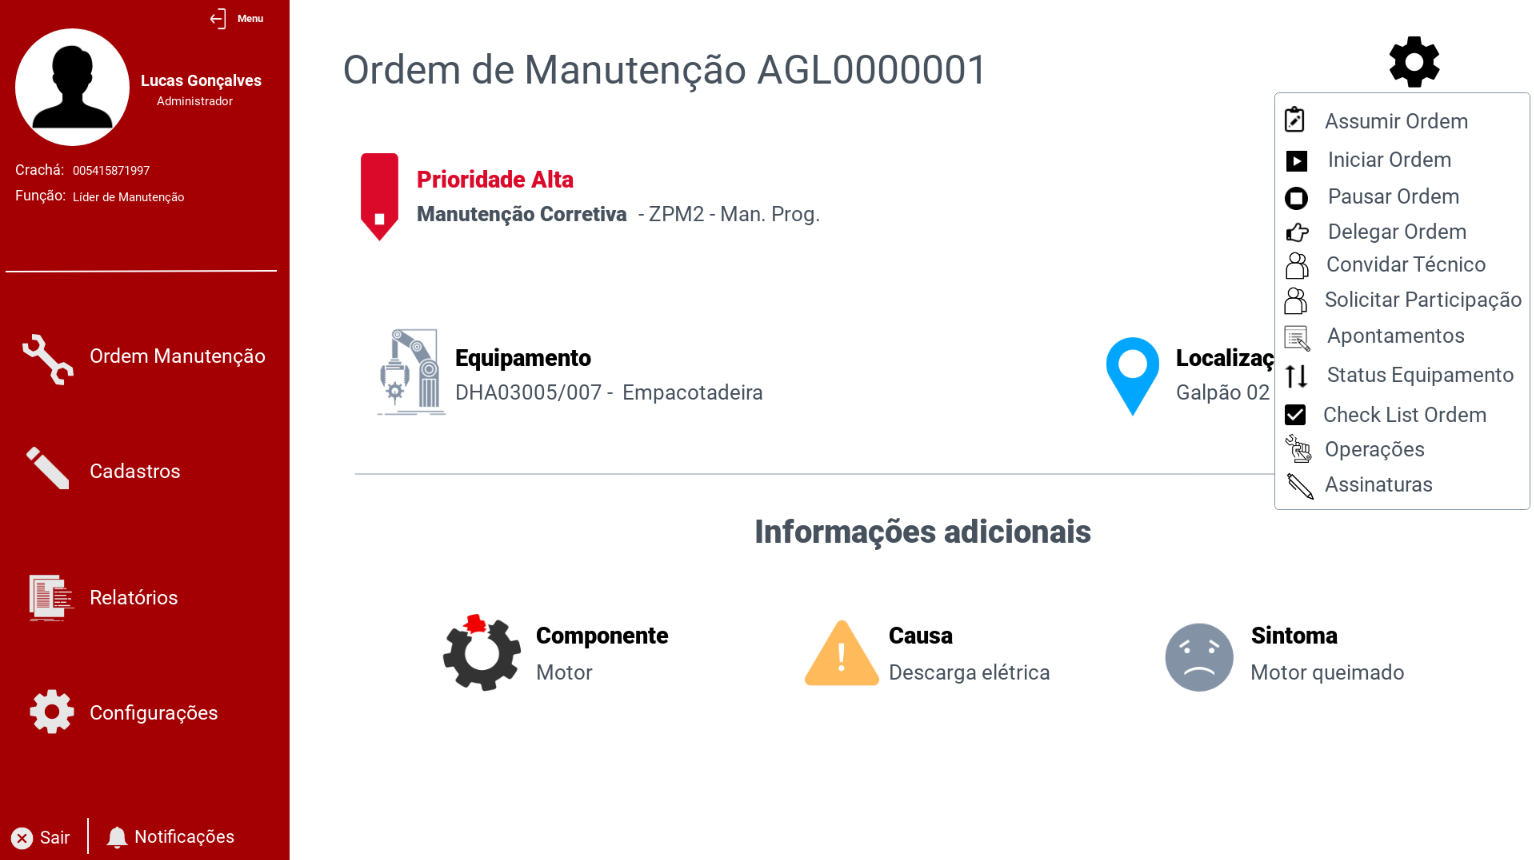
\includegraphics[scale=0.40]{./Figuras/web/om-capa.png}
	\end{center}
	\legend{Fonte: Próprio Autor, 2019}
\end{figure}

Na tela \ref{web_om-capa} será possível acompanhar o andamento de uma ordem de manutenção de lista, ver informações referente à ordem e executar ações nela, como alterar status, adicionar operações e realizar assinaturas.

\newpage
\subsection{Checklist de Segurança}

\begin{figure}[htb]
	\caption{\label{web_check-list}Checklist de Segurança}
	\begin{center}
		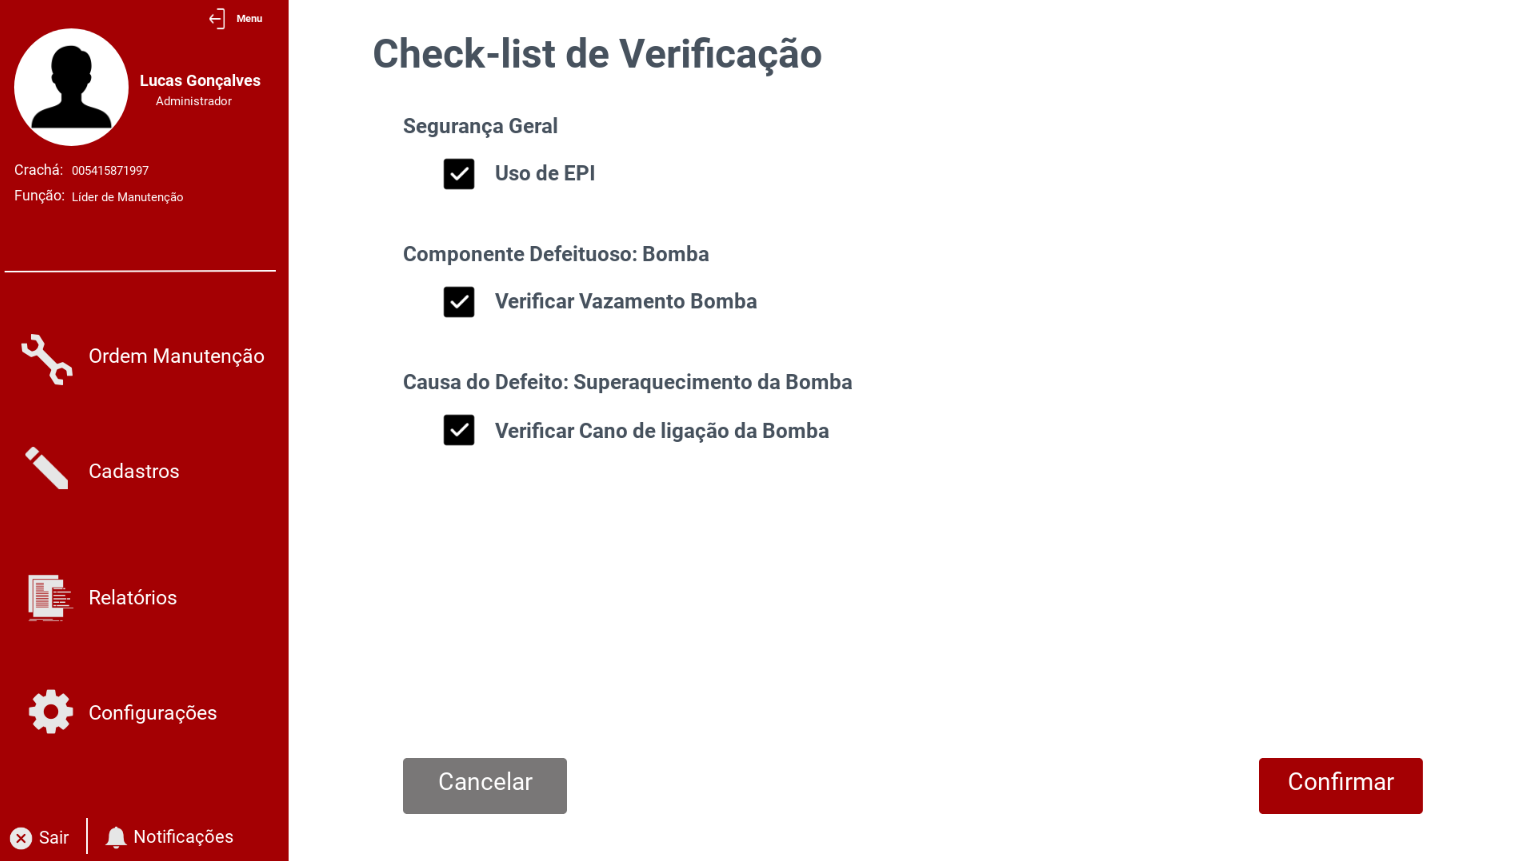
\includegraphics[scale=0.40]{./Figuras/web/check-list.png}
	\end{center}
	\legend{Fonte: Próprio Autor, 2019}
\end{figure}

Na tela \ref{web_check-list} o manutentor irá marcar a lista de segurança antes de iniciar a ordem de manutenção.

\newpage
\subsection{Operações da Ordem de Manutenção}

\begin{figure}[htb]
	\caption{\label{web_om-operacoes}Operações da Ordem de Manutenção}
	\begin{center}
		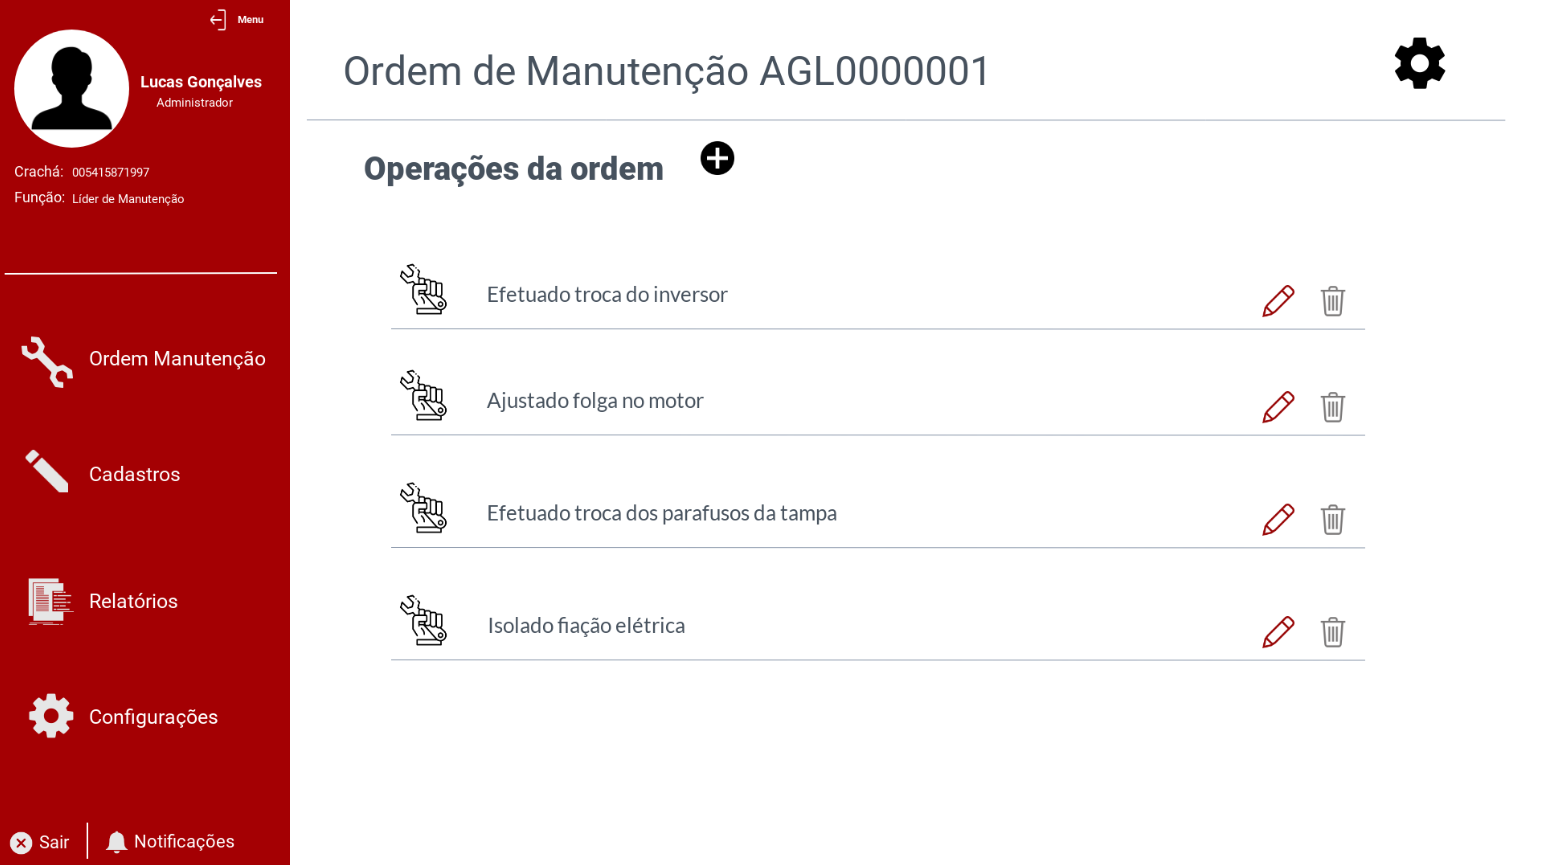
\includegraphics[scale=0.40]{./Figuras/web/om-operacoes.png}
	\end{center}
	\legend{Fonte: Próprio Autor, 2019}
\end{figure}

Na tela \ref{web_om-operacoes} é possível verificar todas as operações pré cadastradas para a OM e cadastrar novas operações conforme necessidade para o andamento da OM.

\newpage
\subsection{Ordem de Manutenção: Lista}

\begin{figure}[htb]
	\caption{\label{web_om-lista}Ordem de Manutenção: Lista}
	\begin{center}
		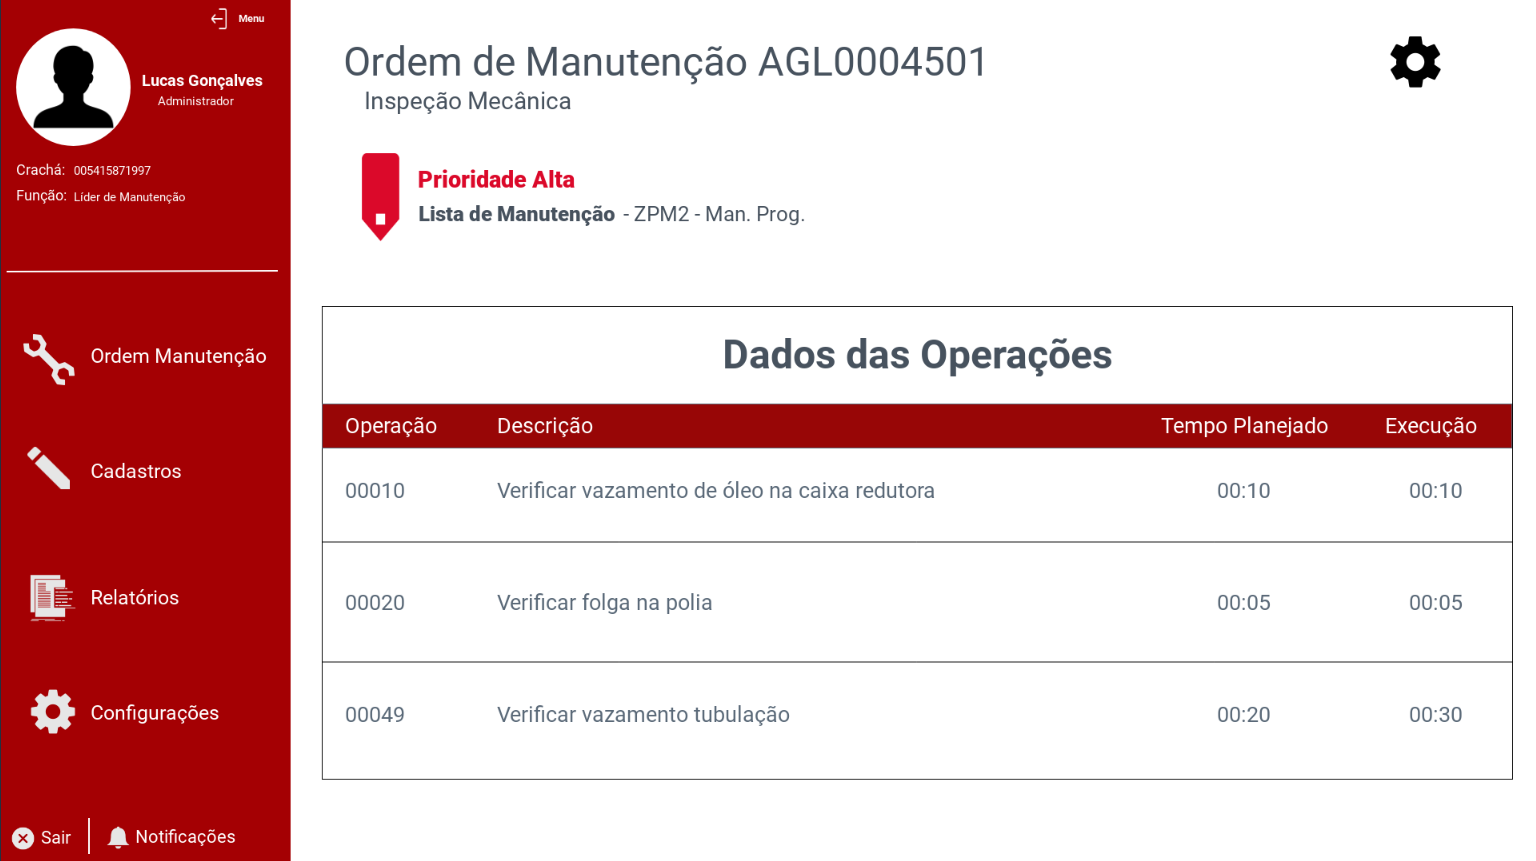
\includegraphics[scale=0.40]{./Figuras/web/om-lista.png}
	\end{center}
	\legend{Fonte: Próprio Autor, 2019}
\end{figure}

Na tela \ref{web_om-lista} será possível acompanhar o andamento de uma ordem de manutenção de lista, ver informações referente à ordem e executar ações nela, como alterar status, adicionar operações e realizar assinaturas.

\newpage
\subsection{Equipamentos da Ordem de Manutenção: Lista}

\begin{figure}[htb]
	\caption{\label{web_om-lista-equipamentos}Equipamentos da Ordem de Manutenção: Lista}
	\begin{center}
		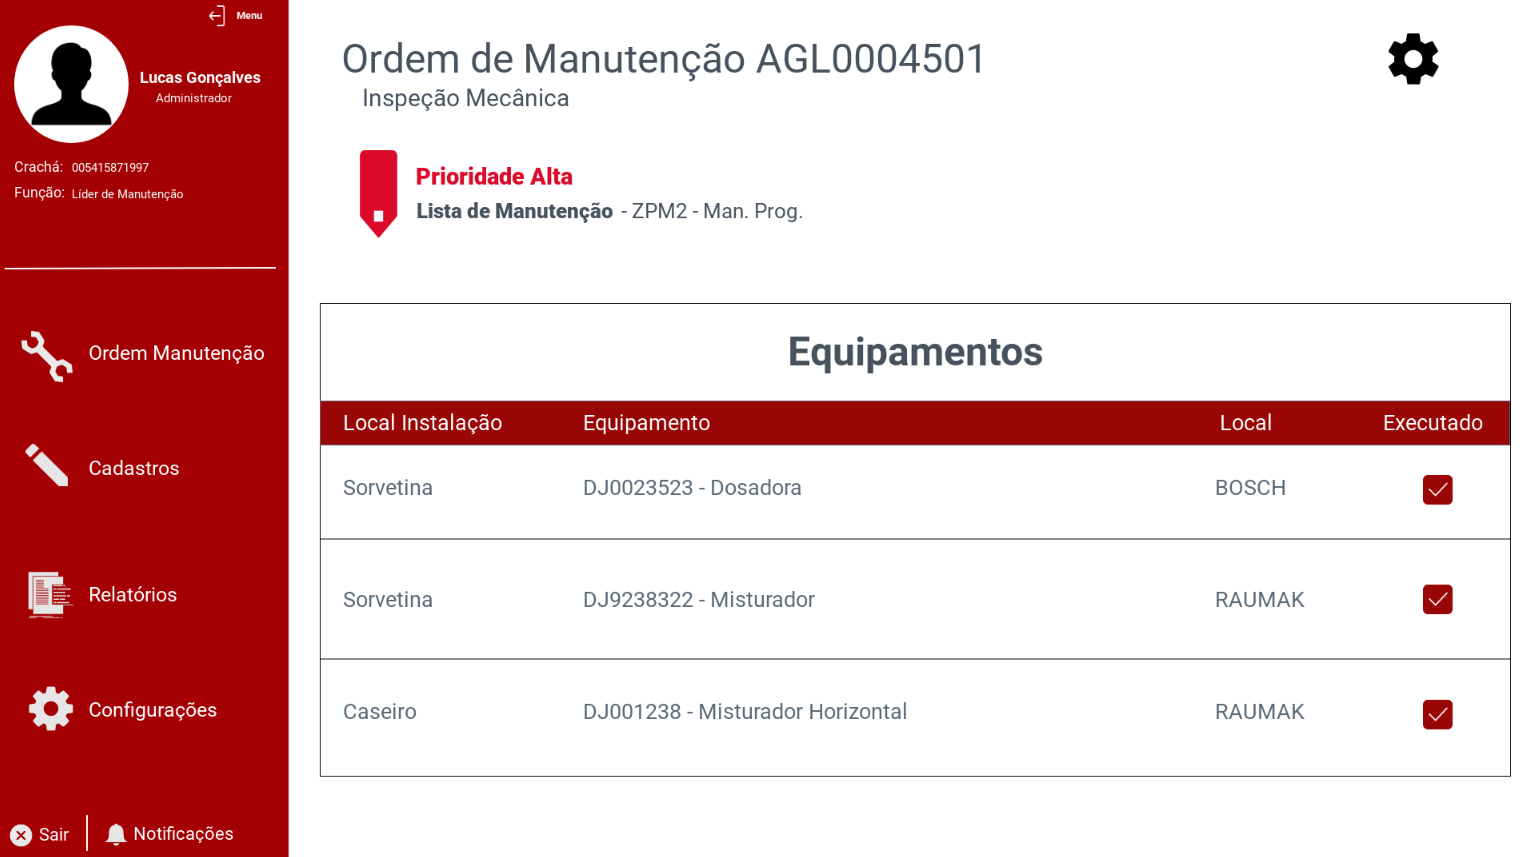
\includegraphics[scale=0.40]{./Figuras/web/om-lista-equipamentos.png}
	\end{center}
	\legend{Fonte: Próprio Autor, 2019}
\end{figure}

Na tela \ref{web_om-lista-equipamentos} será possível acompanhar os equipamentos que terão de ser inspecionados pelo manutentor e o mesmo marcar se executou ou não.

\newpage
\subsection{Ordem de Manutenção: Rota}

\begin{figure}[htb]
	\caption{\label{web_om-rota}Ordem de Manutenção: Rota}
	\begin{center}
		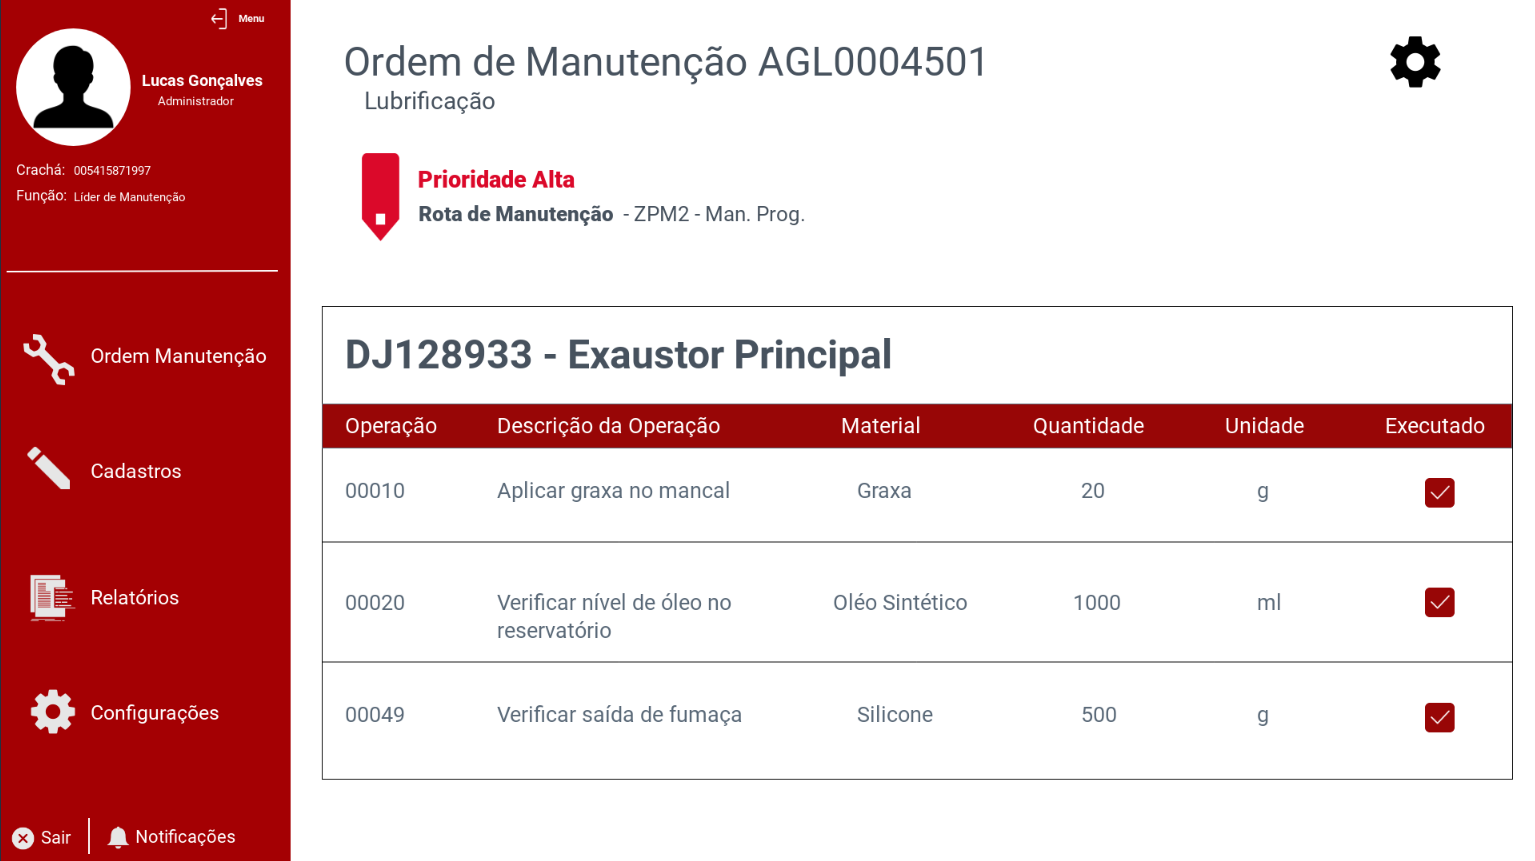
\includegraphics[scale=0.40]{./Figuras/web/om-rota.png}
	\end{center}
	\legend{Fonte: Próprio Autor, 2019}
\end{figure}

Na tela \ref{web_om-rota} será possível acompanhar o andamento de uma ordem de manutenção de lista, ver informações referente à ordem e executar ações nela, como alterar status, adicionar operações e realizar assinaturas.

\newpage
\subsection{Convidar ou Delegar Ordem de Manutenção}

\begin{figure}[htb]
	\caption{\label{web_om-convidar-delegar}Convidar ou Delegar Ordem de Manutenção}
	\begin{center}
		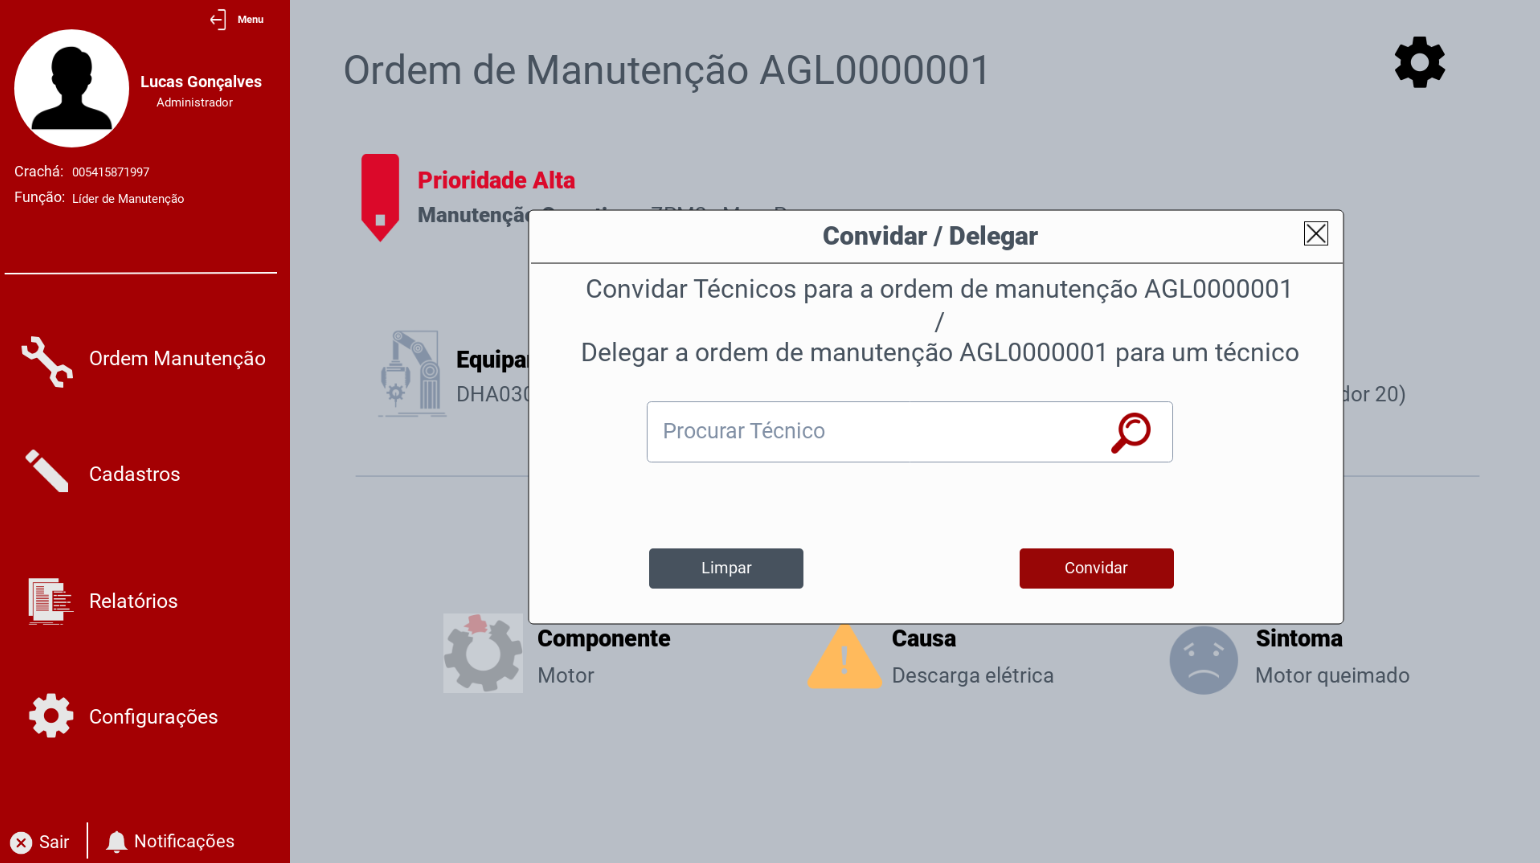
\includegraphics[scale=0.40]{./Figuras/web/om-convidar-delegar.png}
	\end{center}
	\legend{Fonte: Próprio Autor, 2019}
\end{figure}

Na tela \ref{web_om-convidar-delegar} será possível convidar técnicos para se juntarem a ordem de manutenção ou delegar a ordem de manutenção a outro manutentor. Ação só permitida àqueles que são responsáveis pela ordem de manutenção, ou seja, os que assumiram ela.

\newpage
\subsection{Apontamentos}

\begin{figure}[htb]
	\caption{\label{web_om-apontamentos}Apontamentos da Ordem de Manutenção}
	\begin{center}
		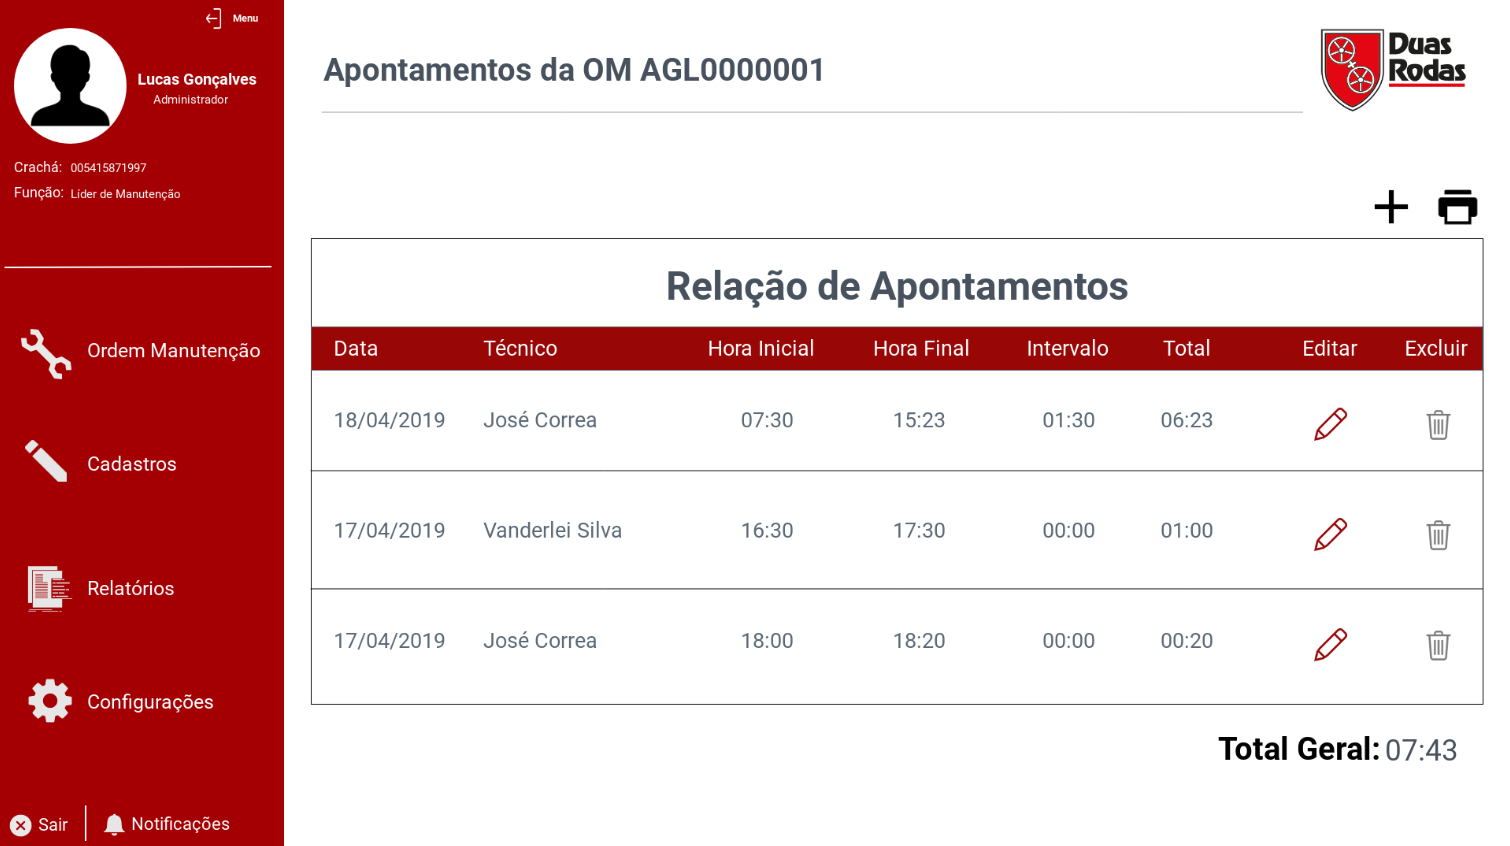
\includegraphics[scale=0.40]{./Figuras/web/om-apontamentos.png}
	\end{center}
	\legend{Fonte: Próprio Autor, 2019}
\end{figure}

Na tela \ref{web_om-apontamentos} será possível visualizar todos os apontamentos que existem em uma ordem, atualizá-las, excluí-las ou adicionar novos apontamentos.

\newpage
\subsection{Adicionar Apontamentos}

\begin{figure}[htb]
	\caption{\label{web_om-add-apontamento}Adicionar Apontamentos na Ordem de Manutenção}
	\begin{center}
		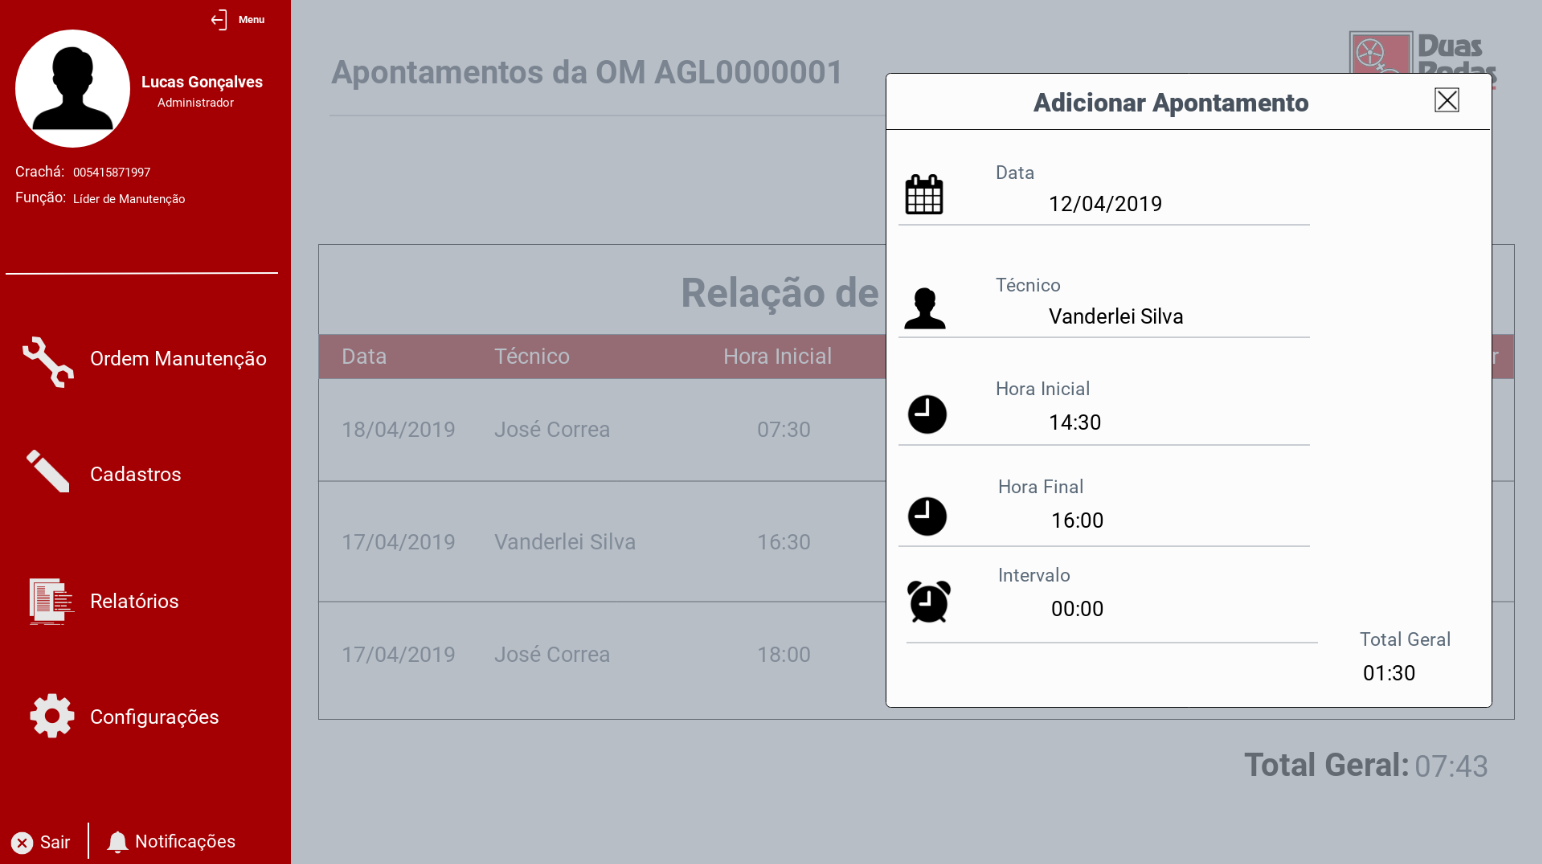
\includegraphics[scale=0.40]{./Figuras/web/om-add-apontamento.png}
	\end{center}
	\legend{Fonte: Próprio Autor, 2019}
\end{figure}

Na tela \ref{web_om-add-apontamento} será possível adicionar novos apontamentos a ordem de manutenção.

\newpage
\subsection{Motivo da Exclusão do Apontamento da Ordem de Manutenção}

\begin{figure}[htb]
	\caption{\label{web_om-excluir-apontamento-motivo}Motivo da Exclusão do Apontamento da Ordem de Manutenção}
	\begin{center}
		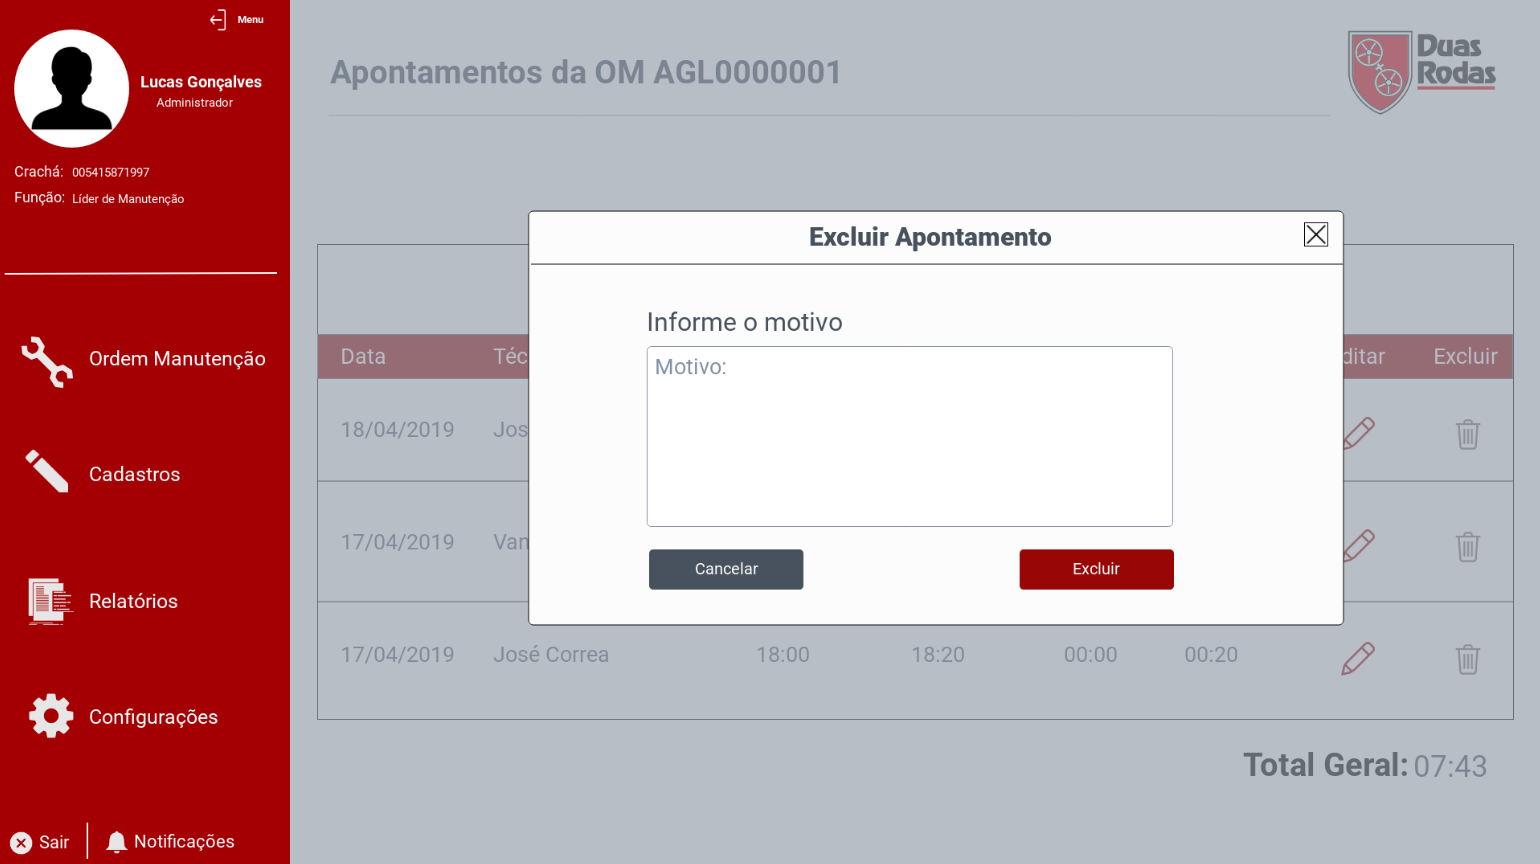
\includegraphics[scale=0.40]{./Figuras/web/om-excluir-apontamento-motivo.png}
	\end{center}
	\legend{Fonte: Próprio Autor, 2019}
\end{figure}

Na tela \ref{web_om-excluir-apontamento-motivo} o operador terá de informar o motivo pela exclusão do apontamento da ordem de manutenção.

\newpage
\subsection{Assinatura Digital}

\begin{figure}[htb]
	\caption{\label{web_om-assinatura}Assinatura Digital}
	\begin{center}
		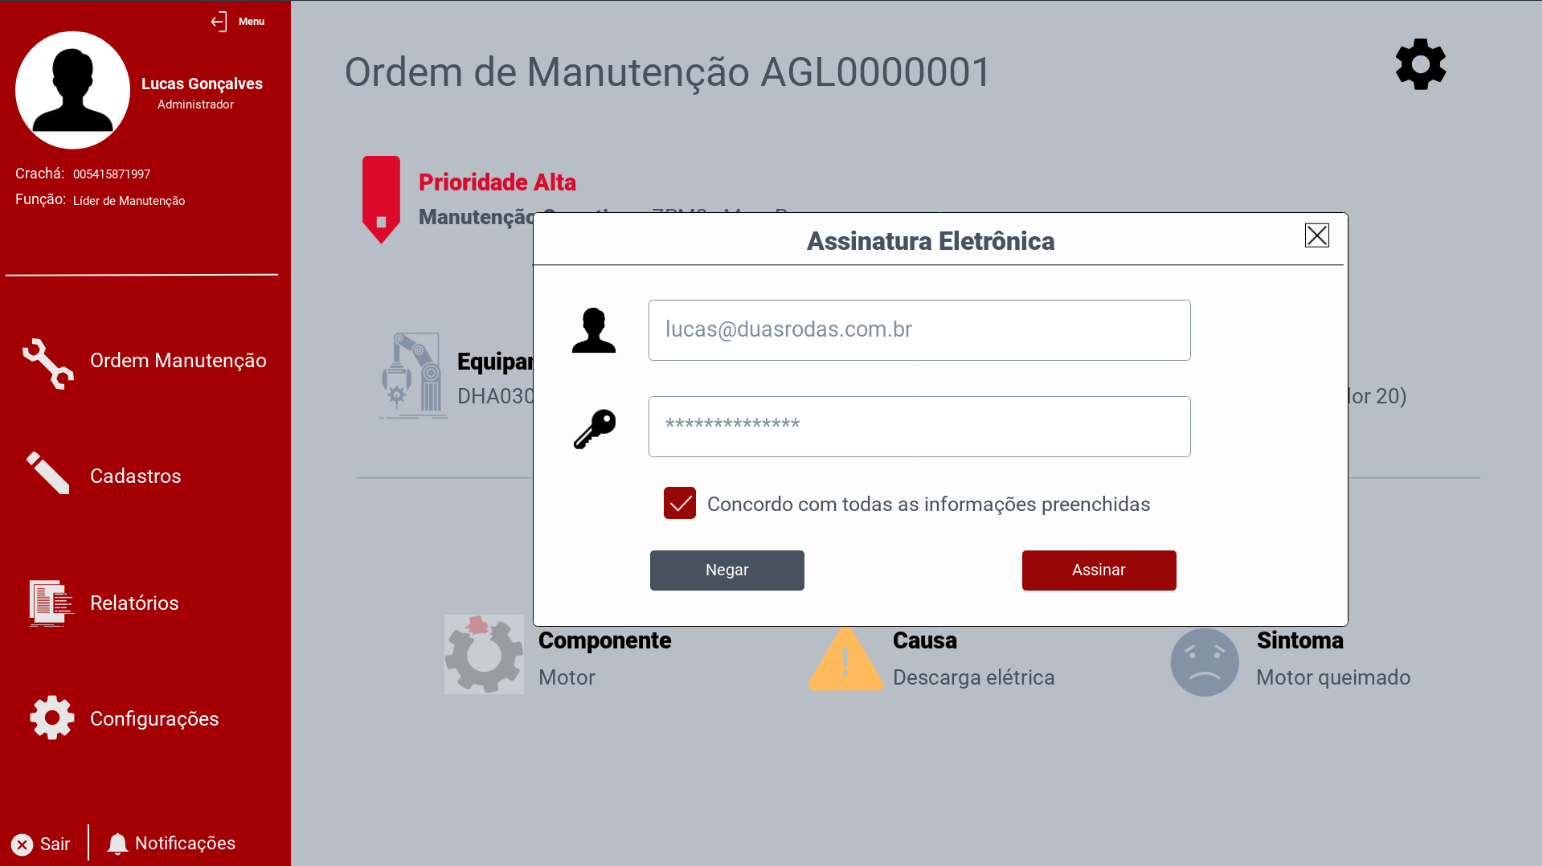
\includegraphics[scale=0.40]{./Figuras/web/om-assinatura.png}
	\end{center}
	\legend{Fonte: Próprio Autor, 2019}
\end{figure}

Na tela \ref{web_om-assinatura} será possível assinar a ordem digitalmente. Para tanto, será cobrado as credenciais do operador.

\newpage
\section{Aplicação Mobile}
A aplicação Mobile é um ponto estratégico do produto, pois sua mobilidade permite com que os técnicos possam atuar na manutenção e realizar anotações e apontamentos no sistema através de um smartphone ou tablet.

\subsection{Login}

\begin{figure}[htb]
	\caption{\label{mobile_login}Login}
	\begin{center}
		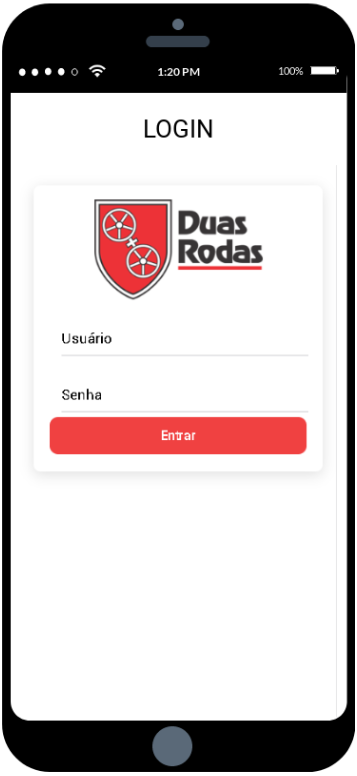
\includegraphics[scale=0.80]{./Figuras/mobile/login.png}
	\end{center}
	\legend{Fonte: Próprio Autor, 2019}
\end{figure}

A tela \ref{mobile_login} será a página responsável por autenticar o usuário e garantir a segurança do sistema.

\newpage
\subsection{Menu}

\begin{figure}[htb]
	\caption{\label{mobile_menu}Menu}
	\begin{center}
		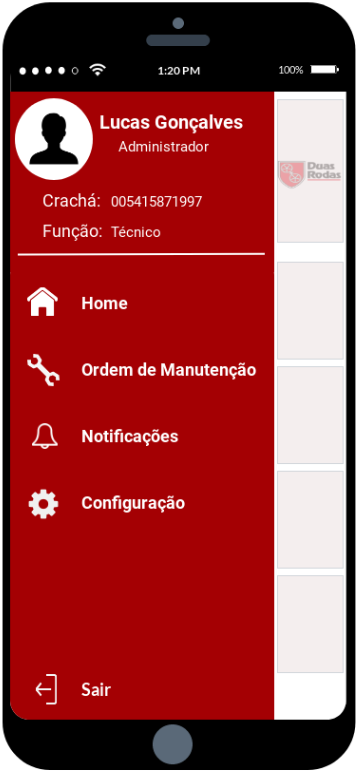
\includegraphics[scale=0.80]{./Figuras/mobile/menu.png}
	\end{center}
	\legend{Fonte: Próprio Autor, 2019}
\end{figure}

A figura \ref{mobile_menu} demonstra o menu lateral do aplicativo, identificando o usuário autenticado e um menu de acesso rápido às principais telas do sistema.

\newpage
\subsection{Monitor}

\begin{figure}[htb]
	\caption{\label{mobile_monitor}Monitor}
	\begin{center}
		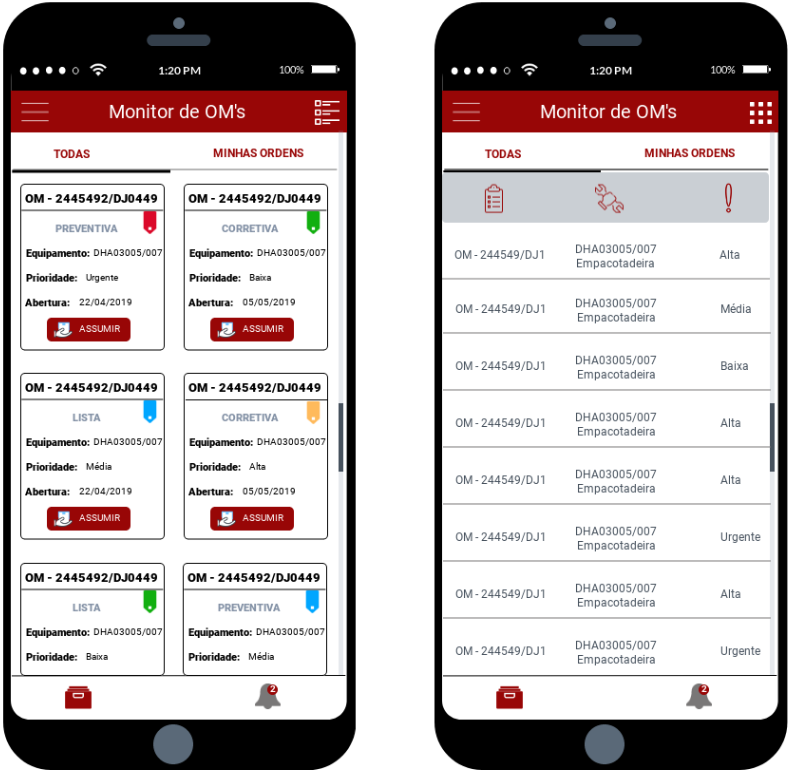
\includegraphics[scale=0.75]{./Figuras/mobile/monitor.png}
	\end{center}
	\legend{Fonte: Próprio Autor, 2019}
\end{figure}

Na figura \ref{mobile_monitor} é possível verificar o monitor do manutentor. Nesse monitor, o manutentor consegue rapidamente visualizar as OMs pendentes e seus respectivos status através das bandeiras indicadas no card. As  vermelhas indicam que a OM tem uma prioridade emergente, as amarelas têm prioridade alta, as azuis têm prioridade média e as verdes possuem uma prioridade baixa.

\newpage
\subsection{Central de Notificações}

\begin{figure}[htb]
	\caption{\label{mobile_notificacao}Notificações}
	\begin{center}
		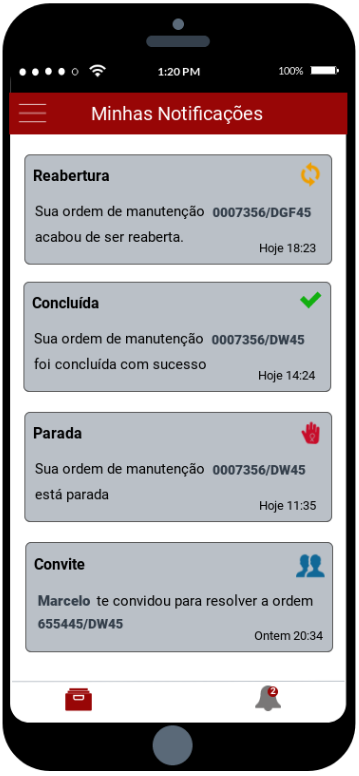
\includegraphics[scale=0.80]{./Figuras/mobile/notificacao.png}
	\end{center}
	\legend{Fonte: Próprio Autor, 2019}
\end{figure}

Na tela \ref{mobile_notificacao} é possível verificar notificações do usuário autenticado no sistema.

\newpage
\subsection{Ordem de Manutenção}

\begin{figure}[htb]
	\caption{\label{mobile_om}Ordem de Manutenção}
	\begin{center}
		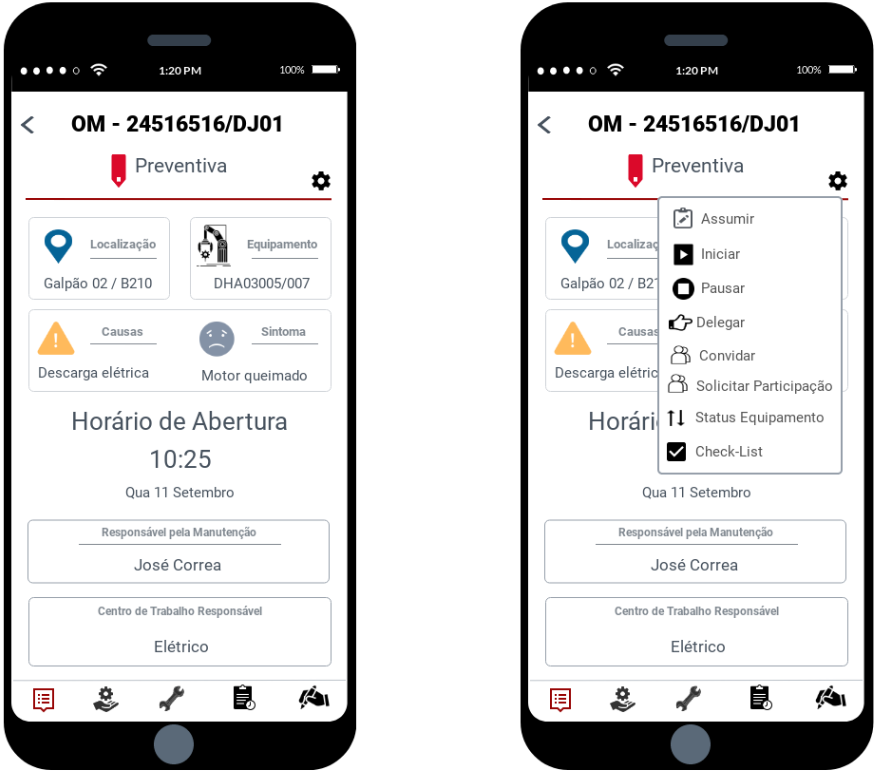
\includegraphics[scale=0.70]{./Figuras/mobile/om.png}
	\end{center}
	\legend{Fonte: Próprio Autor, 2019}
\end{figure}

Na tela \ref{mobile_om} será possível acompanhar o andamento de uma ordem de manutenção preventiva e corretiva, ver informações referente à ordem e executar ações nela, como alterar status, adicionar operações e realizar assinaturas.

\newpage
\subsection{Ordem de Manutenção: Lista}

\begin{figure}[htb]
	\caption{\label{mobile_lista}Ordem de Manutenção: Lista}
	\begin{center}
		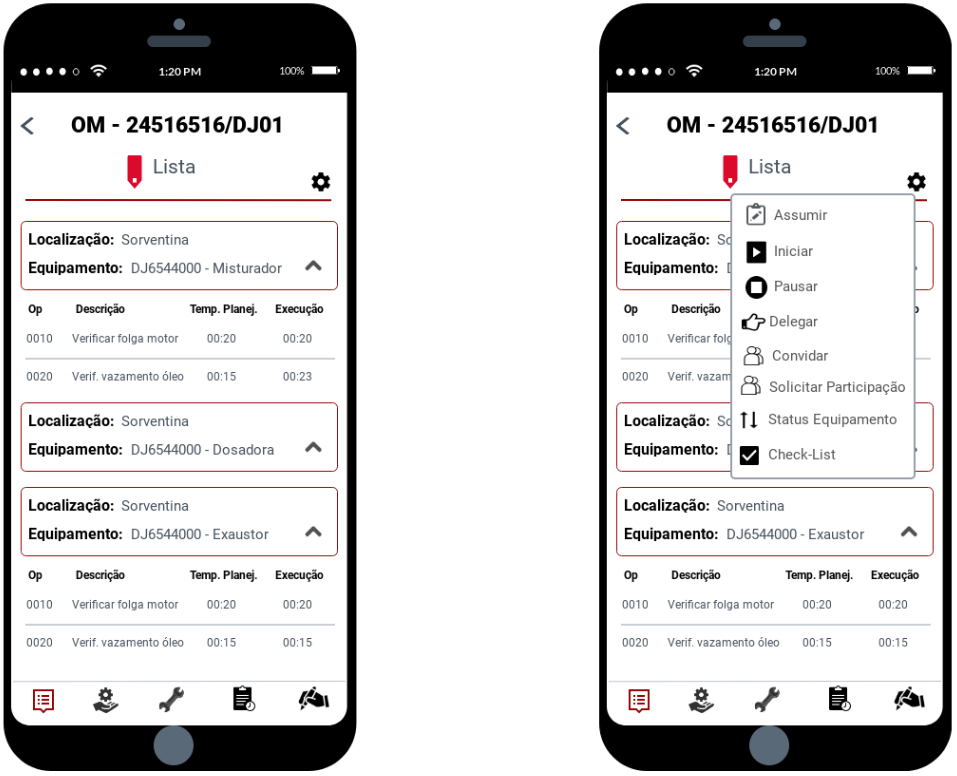
\includegraphics[scale=0.65]{./Figuras/mobile/lista.png}
	\end{center}
	\legend{Fonte: Próprio Autor, 2019}
\end{figure}

Na tela \ref{mobile_lista} será possível acompanhar o andamento de uma ordem de manutenção de lista, ver informações referente à ordem e executar ações nela, como alterar status, adicionar operações e realizar assinaturas.

\newpage
\subsection{Ordem de Manutenção: Rota}

\begin{figure}[htb]
	\caption{\label{mobile_rota}Ordem de Manutenção: Rota}
	\begin{center}
		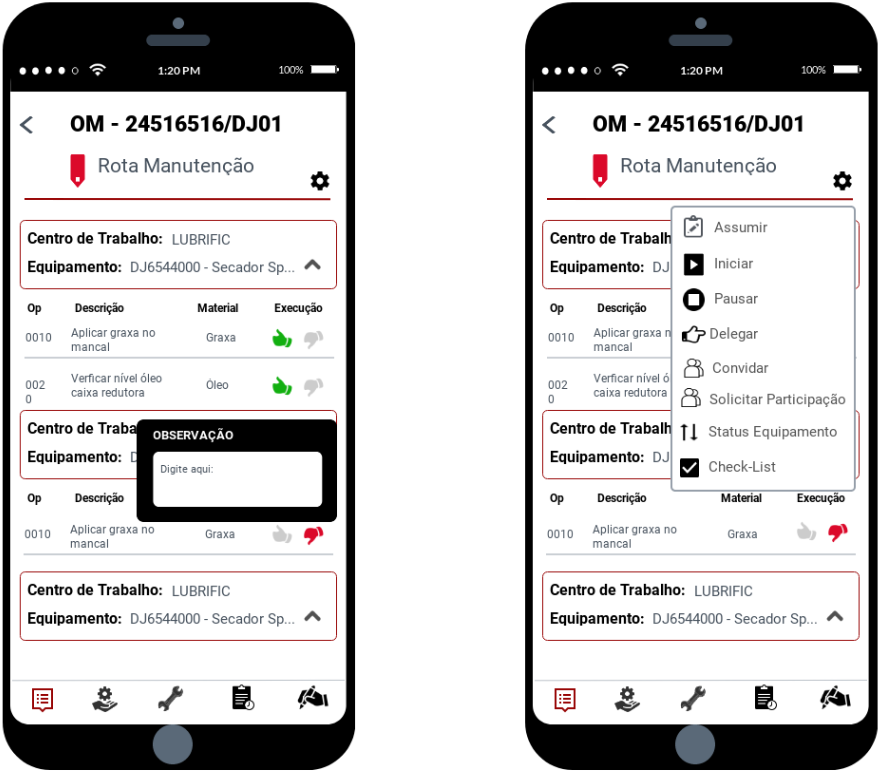
\includegraphics[scale=0.70]{./Figuras/mobile/rota.png}
	\end{center}
	\legend{Fonte: Próprio Autor, 2019}
\end{figure}

Na tela \ref{mobile_rota} será possível acompanhar o andamento de uma ordem de manutenção de rota, ver informações referente à ordem e executar ações nela, como alterar status, adicionar operações e realizar assinaturas.

\newpage
\subsection{Checklist de Segurança}

\begin{figure}[htb]
	\caption{\label{mobile_checklist}Checklist de Segurança}
	\begin{center}
		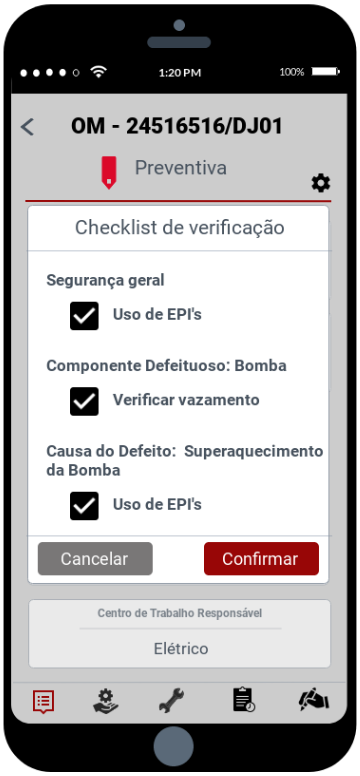
\includegraphics[scale=0.80]{./Figuras/mobile/checklist.png}
	\end{center}
	\legend{Fonte: Próprio Autor, 2019}
\end{figure}

Na tela \ref{mobile_checklist} o manutentor irá marcar a lista de segurança antes de iniciar a ordem de manutenção.

\newpage
\subsection{Problemas}

\begin{figure}[htb]
	\caption{\label{mobile_problema}Problemas}
	\begin{center}
		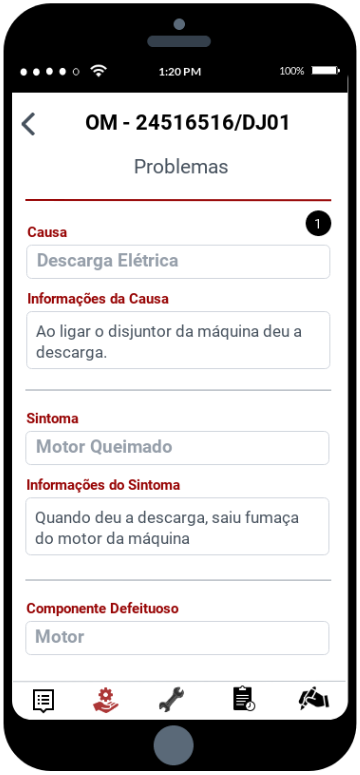
\includegraphics[scale=0.80]{./Figuras/mobile/problemas.png}
	\end{center}
	\legend{Fonte: Próprio Autor, 2019}
\end{figure}

Na tela \ref{mobile_problema} o manutentor irá verificar com maiores detalhes os problemas identificados no equipamento.

\newpage
\subsection{Componentes}

\begin{figure}[htb]
	\caption{\label{mobile_componentes}Componentes da Ordem de Manutenção}
	\begin{center}
		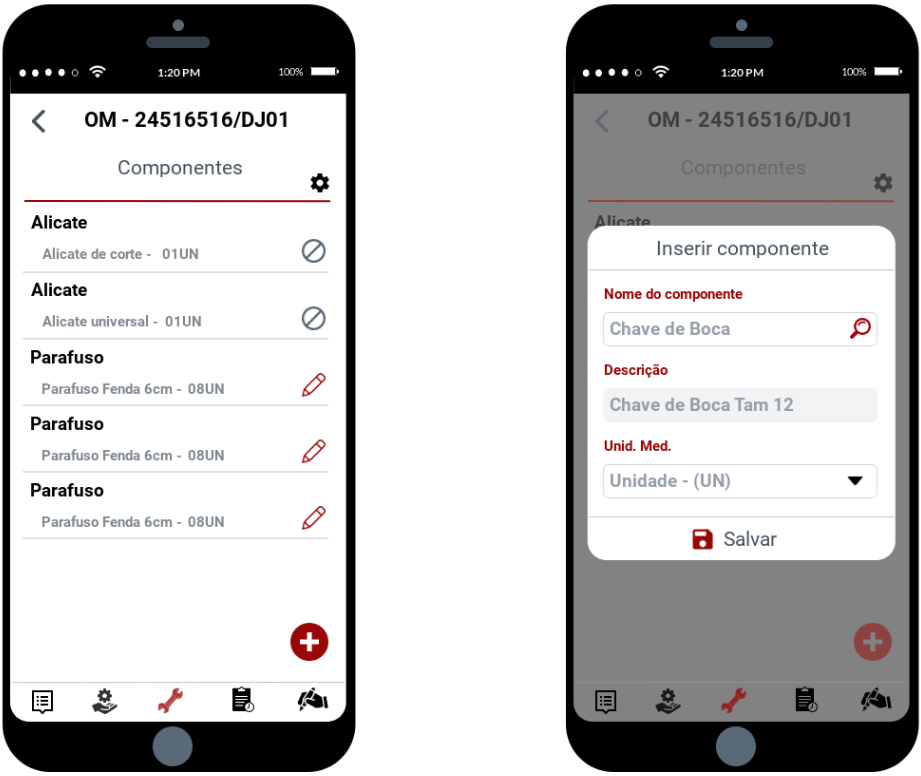
\includegraphics[scale=0.70]{./Figuras/mobile/componentes.png}
	\end{center}
	\legend{Fonte: Próprio Autor, 2019}
\end{figure}

Na tela \ref{mobile_componentes} é possível verificar todos os componentes utilizados na operação da ordem de manutenção.

\newpage
\subsection{Operações}

\begin{figure}[htb]
	\caption{\label{mobile_operacao}Operações da Ordem de Manutenção}
	\begin{center}
		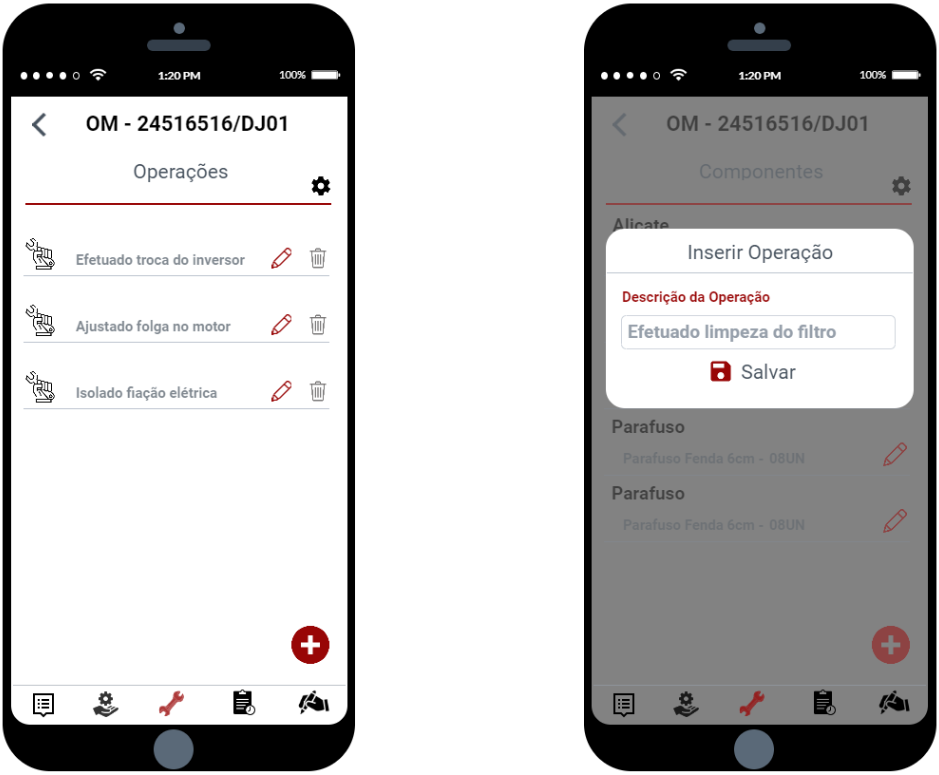
\includegraphics[scale=0.70]{./Figuras/mobile/operacao.png}
	\end{center}
	\legend{Fonte: Próprio Autor, 2019}
\end{figure}

Na tela \ref{mobile_operacao} é possível verificar todas as operações pré cadastradas para a OM e cadastrar novas operações conforme necessidade para o andamento da OM.

\newpage
\subsection{Apontamentos}

\begin{figure}[htb]
	\caption{\label{mobile_apontamentos}Apontamentos da Ordem de Manutenção}
	\begin{center}
		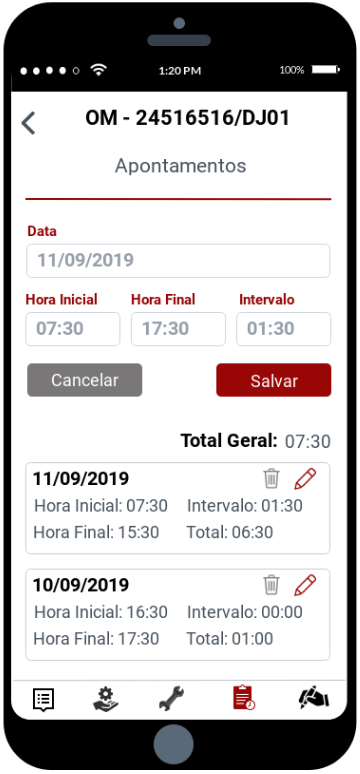
\includegraphics[scale=0.80]{./Figuras/mobile/apontamentos.png}
	\end{center}
	\legend{Fonte: Próprio Autor, 2019}
\end{figure}

Na tela \ref{mobile_apontamentos} é possível realizar os apontamentos das horas trabalhadas na execução da ordem de manutenção.

\newpage
\subsection{Assinatura Digital}

\begin{figure}[htb]
	\caption{\label{mobile_assinaturas}Assinatura Digital}
	\begin{center}
		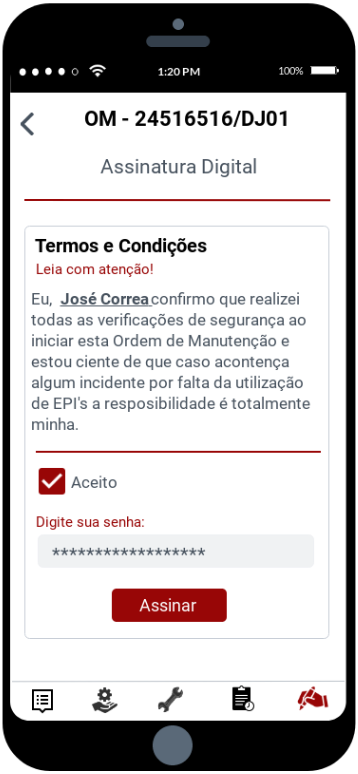
\includegraphics[scale=0.80]{./Figuras/mobile/assinaturas.png}
	\end{center}
	\legend{Fonte: Próprio Autor, 2019}
\end{figure}

Na tela \ref{mobile_assinaturas} é possível verificar e realizar as assinaturas.